\part{Mise en œuvre et couplage relationnel}
La définition d'Astral nous permet de créer des requêtes pouvant manipuler toutes les données des systèmes observés. Cette partie présente l'exécution de ces requêtes. Nous dédions un chapitre à l'intergiciel Astronef qui est un système de gestion de flux de données extensible. Ceci forme une bonne base de travail, car il est possible d'ajouter facilement des composants, ce que nous faisons pour ajouter l'utilisation d'un support persistant relationnel avec Asteroid. De plus, nous proposons un schéma conceptuel de base de données pour utiliser ce support lors de l'observation de systèmes.

\begin{savequote}[6cm]
<< Is this thing on? I don't think this thing is on. Hello! [...] Confangled modern doohickeys. >>
\qauthor{Grany Smith}
\end{savequote}

\chapter{Astronef : De l'expression à l'exécution}\label{chap:contrib:astronef}
\chaptertoc

\lstset{language=PrologAstral}
\section{De l'algèbre aux composants}\label{sec:contrib:astronef:architecture}
Dans cette section, nous détaillons les éléments d'architectures que nous avons mis en œuvre pour permettre à une requête Astral d'être instanciée en un processus de traitement. Nous abordons premièrement les principes architecturaux utilisés. Ensuite, nous détaillons les différents composants utilisés dans Astronef. Enfin, nous présentons notre méthode extensible de construction de plan par l'utilisation d'un système de règles.
\subsection{Architecture}
Avant de détailler l'architecture de notre système de traitement de requêtes continues, nous allons d'abord présenter le paradigme architectural dans lequel nous allons mettre en œuvre Astronef. Nous présentons premièrement et brièvement les architectures à services. Puis, nous détaillons les principes des architectures à composants orientés services que nous utilisons par la suite.
\subsubsection{Architecture à service}
Les architectures à services permettent aux applications d'être assemblés sous forme de blocs réutilisables étant des \textit{services}. Un \textit{service} est définit par une spécification (ou \textit{description}, ou \textit{contrat}), qui décrit sa syntaxe, son comportement, sa sémantique ainsi que sa dépendance aux autres services. Dans les architectures à service, les services interagissent via un patron récurrent d'interaction (fig~\ref{fig:contrib:astronef:services}). 
\begin{figure}[ht]
    \centering
    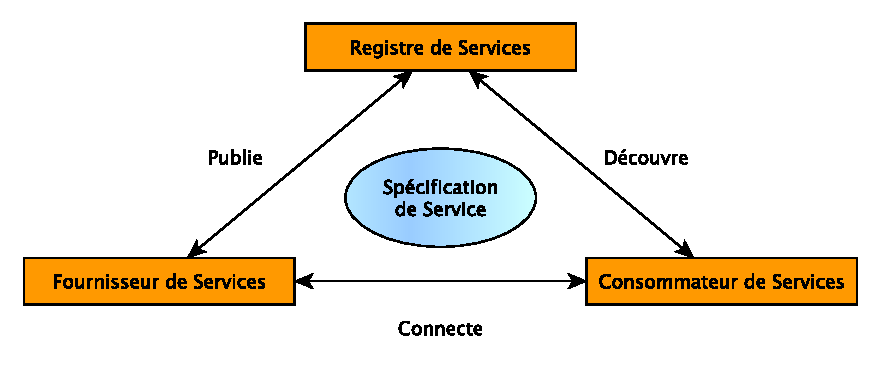
\includegraphics[width=0.7\textwidth]{contrib-astronef-services}
    \caption{Patron d'interaction de service}\label{fig:contrib:astronef:services}
\end{figure}
Un fournisseur de service va publier sa spécification à un registre. Un consommateur de service découvre le service fournit par une requête sur le registre. Enfin, le consommateur et le fournisseur se connectent. Le point clé de cette architecture étant que cette résolution est faite au \textit{runtime}.

\subsubsection{Architecture à composants orientés services}
Le modèle d'architecture à composants orientés services~\cite{Cervantes:servicecomponent} permet la mise en œuvre d'applications à base de services dans le paradigme de la programmation par composants. Le principe étant de séparer les mécanismes des architectures à services du code implémentant le comportement du service fournit. Ainsi, voici les principes d'un tel modèle :
\begin{itemize}
    \item Un service est une fonctionnalité fournie.
    \item Un service est caractérisé par sa spécification.
    \item Les composants implémentent des spécifications de services, qui peuvent eux-mêmes dépendre, du fait de leurs implémentations, d'autres services.
    \item Les patrons d'interactions de services sont utilisés pour résoudre les dépendances de services au \textit{runtime}.
    \item Les compositions sont décrites en terme de spécifications de services.
    \item Tout composant peut se substituer par un autre si les spécifications de services sont identiques.
\end{itemize}
Nous mêlons donc dans un même modèle, les idées de composants et de services. De plus, en s'inspirant des modèles récents tels que Fractal~\cite{Bruneton:fractal}, chaque composant possède un ensemble de propriétés (ou attributs) configurables. Nous obtenons aussi le pouvoir d'instancier (grâce aux fabriques) des composants à partir de configurations.

\begin{figure}[ht]
    \centering
    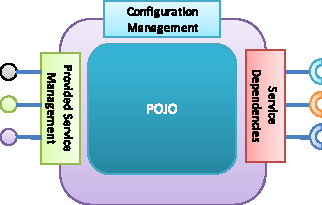
\includegraphics[width=0.5\textwidth]{contrib-astronef-ipojo}
    \caption{Un composant iPojo}\label{fig:contrib:astronef:ipojo}
\end{figure}
La figure~\ref{fig:contrib:astronef:ipojo} représente un composant dans l'implémentation \textit{iPojo}~\cite{Escoffier:ipojo}. Le principe étant que le code du composant (le \textit{POJO}, \textit{Plain Old Java Object}) est embarqué dans un conténaire auxquels seront accrochés des gestionnaires. Les trois couramment utilisés sont les gestionnaires de dépendances, de production de service, et de configuration. Ainsi, un composant pourra s'exposer sur un registre, tout en dépendant d'autres services et en supportant le fait d'être configurable.

\subsection{Les différents composants et services}
L'architecture d'Astronef est entièrement dirigé par ces approches. De multiples composants sont ainsi créés et instantiables, pour former une requête. Afin de pouvoir exécuter les requêtes, nous définissons trois services centraux :
\begin{itemize}
	\item[\textbf{Les \textit{EventProcessor}}] : Ces services ont deux primitives, l'une exécute une tâche quelconque, l'autre indique les autres \textit{EventProcessors} dont il dépend.
	\item[\textbf{Le \textit{Scheduler}}] : Ce service permet la planification. Ses primitives permettent aux différents \textit{EventProcessor} d'exprimer leur volonté de s'exécuter. Ce service devra mettre en ordre ces demandes en fonction des dépendances exprimés.
	\item[\textbf{Le \textit{QueryRuntime}}] : Ce service permet d'exécuter une requête. Il est lié à un \textit{Scheduler}, et utilise la primitive \textit{next} de celui-ci pour connaître la prochaine tâche qu'il faudra exécuter.
\end{itemize}

Nous adoptons ainsi l'approche émise par~\cite{Carney:scheduling} pour gérer l'ordonnancement des événements. Maintenant que nous avons vu les différents services nécessaire à l'exécution. Nous avons plusieurs types de composants que nous pourrons instantier :
\begin{itemize}
	\item[\textbf{Les entités}] : Fournissent les services nécessaires pour manipuler un flux ou une relation. Ces entités servent de résultats intermédiaires (ou de tampons). De plus, ils permettent un service de notification. En cas de changement, les \textit{EventProcessor} abonnés seront notifiés. Ainsi, ces composants nécessitent un \textit{Scheduler} pour demander l'exécution de leurs abonnés.
	\item[\textbf{Les sources}] : Une source nécessite une entité en lecture, dont elle manipulera le contenu pour la remplir. Ce composant pourra nécessiter le \textit{Scheduler} pour, entre autres, notifier la fin de son envoi et donc la fin de la requête.
	\item[\textbf{Les opérateurs}] : Nécessitent $n$ entités en lecture, et une autre particulière en écriture. Ce composant doit fournir le service \textit{EventProcessor}. Les implémentations des opérateurs bloquants pourront faire appel au \textit{Scheduler} pour planifier des exécutions ponctuelles.
	\item[\textbf{Les puits}] : Nécessitent une entité en lecture. Ce composant fournit le service \textit{EventProcessor} et doit être non-bloquant (donc seulement s'abonner à son entité en lecture).
\end{itemize}

Ainsi pour créer une requête : l'utilisateur doit fournir un ou plusieurs composants sources et un composant puit. Par la suite, il demande à Astronef de lui instantier ses sources et son puit en configurant les composants selon sa volonté. Enfin, il spécifie l'expression algébrique liant les sources au puit.

\subsubsection{De l'importance de la réutilisation}
Le fait d'abstraire l'architecture d'\textit{Astronef} permet une grande flexibilité architecturale. Tout d'abord, pour chaque composant, le fait de pouvoir le configurer tout en gérant son cycle de vie permet de réutiliser le même module pour plusieurs usages. Par exemple, supposons l'existance d'une source capable de récupérer une information périodiquement sur un protocole donné. Cette source pourra être utilisé pour plusieurs requêtes sous différentes instances en ayant plusieurs configurations.

Mais cette abstraction sous forme de services permet surtout la substitution. En effet, nous pouvons remplacer n'importe quel composant du moment qu'il supporte le même service. Nous utilisons ce principe pour sélectionner les meilleurs composants pour remplir le plus efficacement leurs rôles. De plus, l'utilisateur peut apporter ses propres implémentations pour étendre les capacités de l'intergiciel.

\subsection{Construction du plan par règles}
Nous définissons un plan de requête comme un ensemble de composants déployés pour répondre à la requête de l'utilisateur. Nous souhaitons avant tout que l'utilisateur n'ai pas à intervenir lors de cette construction. De son point de vue, il ne doit écrire que l'expression algébrique de sa requête et il doit être garanti d'une mise en œuvre efficace.

Pour atteindre ce but, nous avons choisi de mettre en place un moteur de règle. Le principe étant que nous partons de l'expression algébrique, puis nous itérons suivant plusieurs schéma d'inférences jusqu'à obtenir un plan de requête. Nous remarquons plusieurs avantage à une telle approche :
\begin{itemize}
	\item Intégration naturelle des connaissances. L'algèbre est pleine de propriété et de théorèmes. Il est nécessaire de pouvoir les exprimer dans un langage déclaratif pour les exploiter et pour en rajouter le plus possible.
	\item Expression de la sémantique des composants par l'algèbre. Comme il est nécessaire d'associer des composants logiciels à la sémantique d'Astral, il est nécessaire de spécifier à quelle opération chaque composant (et chaque paramètre de configuration) répond. Cela permet une clarification des sémantiques d'exécution.
	\item Extensibilité très forte. En considérant que l'ajout de nouveaux composants peut se faire via l'ajout de nouvelles règles, il devient aisé d'étendre le système pour permettre des opérateurs, ou des optimisations qui n'étaient pas prévues.
\end{itemize}

Afin de mettre en œuvre cet ensemble de règle pour obtenir un plan de requête efficace, nous faisons une analogie avec les systèmes de gestions de base de données. Comme présenté dans la section~\ref{sec:rw:sgfd:optim}, l'optimisation est découpé en deux parties : l'optimisation logique, et l'optimisation physique. Nous réutiliserons cette approche qui a fait ses preuves au fur et à mesure des années. Nous restructurerons donc la structure de l'expression algébrique dans la section~\ref{sec:contrib:astronef:logique} pour qu'elle soit plus optimisé. Ensuite, nous sélectionnerons les meilleurs composants et les meilleures configurations pour mettre en œuvre cette nouvelle expression, dans la section~\ref{sec:contrib:astronef:physique}.

Nous utilisons un moteur capable d'exécuter du Prolog~\footnote{En réalité, le langage utilisé (PROVA~\cite{Kozlenkov:prova}) est un dérivé de Prolog mieux adapté à l'intégration avec Java. Mais le principe reste tout à fait similaire.}, langage de programmation logique, pour appliquer nos règles. Avant de détailler l'ensemble de ces règles, nous présentons d'abord la structure d'une expression. Toute expression étant structuré sous forme d'arbre, il est possible de représenter une requête avec des nœuds de la forme\footnote{L'utilisation d'objets de propriétés fait partie du langage PROVA, mais cela reste formalisable en Prolog standard avec une liste d'éléments [clé,valeur].} :
\begin{center} [$\underbrace{A}_{\textrm{Nature du nœud}}$, $\underbrace{B}_{\textrm{Ensemble de propriétés}}$, $\underbrace{C}_{\textrm{Liste de nœuds fils}}$] \end{center}
\begin{example}
	Soit $R$ une source déclaré dans le système, nous souhaitons exécuter la requête $\sigma_{id=1} R$. Alors l'expression de cette requête est la suivante :
	\begin{lstlisting}
[sigma,	{"condition":"id=1"}, [
	[source, {id:"R"}, []]
]]
	\end{lstlisting}
\end{example}
Nous remarquons que cette syntaxe est très similaire au \textit{XML}, c'est pour cela que ce langage est celui utilisé en pratique pour spécifier des requêtes dans le prototype. Il est ensuite traduit en expression utilisable en Prolog. L'ensemble des nœuds possibles corresponds aux différents opérateurs de l'algèbre. Nous ne détaillerons pas ceci dans ce manuscrit. Le lecteur pourra consulter le manuel sur la page web suivante \url{http://code.google.com/p/astral/wiki/XMLSyntax} pour trouver les expressions exactes supportées.
\section{Optimisation logique}\label{sec:contrib:astronef:logique}
Cette première application de règles permet de restructurer l'expression de la requête pour avoir la structure la plus adéquate. Dans cette section, nous pourrons exploiter les connaissances accumulés dans les théorèmes d'Astral que nous pourrons retrouver dans le chapitre~\ref{chap:validation:expressivite}.
\subsection{Préparation}
Tout d'abord, il est nécessaire d'appliquer les sucres syntaxiques pouvant être présents dans l'expression. Par exemple, l'opérateur $\ssjoin$ est un opérateur composite qui n'est défini que par la composition d'autres opérateurs primitifs.

\begin{regle}[Sucres syntaxiques]
L'application de sucre syntaxique transformant l'expression $[A1,B1,C1]$ en $[A2,B2,C2]$ se fait par le prédicat :
\begin{center} \textbf{sugar}($[A1,B1,C1]$, $[A2,B2,C2]$).\end{center}
Ce prédicat est appliqué tant qu'il peut l'être (de manière itérative).
\end{regle}

\begin{example}
	Nous nous proposons d'appliquer le sucre syntaxique pour transformer $\Join_c$ en $\sigma_c \Join$. Pour rappel, le prédicat \textit{sugar} sera appliqué si et seulement si ses conditions sont vérifiées. Ici, nous vérifions qu'il y a une condition \textit{Cond} dans les propriétés. Par la suite, nous pouvons transformer la jointure en sélection-jointure (après avoir retiré la condition des propriétés évidemment).
	\begin{lstlisting}[language=Prolog]
sugar(
	[join,B,C], 
	[sigma, {"condition": Cond}, [
		[join,BOut,C]
	]]
):-
    	map_get(B, "condition", Cond), %La jointure est avec condition
    	!, % alors...
    	map_remove(B, "condition", BOut). %Suppression de la condition
	\end{lstlisting}
\end{example}

Maintenant, afin de pouvoir traiter correctement les différents nœuds, il nous faut inférer les deux propriétés majeures de chaque nœud d'une requête qui va définir la nature de son résultat intermédiaire : son type (\textit{flux} ou \textit{relation}) et ses attributs. Pour cela, il faut être garanti que les sources exposent leurs attributs et types dans leurs propriétés. Par la suite, un programme appliquera ces règles de façon récursive. Les résultats seront stockés dans les propriétés \textit{type} et \textit{attributes}.

\begin{regle}[Inférences de types et d'attributs]
L'inférence du type $Type$ de l'expression $[A,B,C]$ dont les types fils sont $TypesFils=[T1,...]$ se fait par le prédicat :
\begin{center} \textbf{typerules}($[A,B,C,TypesFils]$, $Type$).\end{center}
De façon similaire, nous obtenons pour la liste d'attributs d'un nœud :
\begin{center} \textbf{attribrules}($[A,B,C,AttributsFils]$, $Attributs$).\end{center}
Ceux deux prédicats s'appliquent de manière récursive, d'abord la projection puis la sélection.
\end{regle}


\begin{example}
	Pour la définition de la jointure, les règles sont simples. Le liste des attributs est l'union des listes d'attributs fils. Et le type est du relationnel vers le relationnel.
	\begin{lstlisting}[language=Prolog]
typerules([join,_,_, TypesFils], Type):- 
	allequal(TypesFils,Type), % Verification que tous soient relationnels 
	relation(Type), !.
attribrules([join,_,_,AttributsFils], Attributs):- !, 
	union(AttributsFils,Attributs).
	\end{lstlisting}
\end{example}

Nous avons maintenant un arbre prêt à être optimisé. Tout d'abord, appliquons les règles les plus classiques dans l'optimisation de requêtes en gestion de base de données : la projection.

\subsection{Projection et sélection}
Cette optimisation permet de réduire l'empreinte mémoire des résultats intermédiaires ce qui de plus réduira les temps de calculs des opérateurs. Pour atteindre ce résultat, il est nécessaire d'appliquer les résultats que nous donne Astral. Ces résultats seront tous présentés dans le chapitre~\ref{chap:validation:expressivite}. Nous pouvons tout de même présenter le prédicat logique qui devra appliquer ces règles.
\begin{regle}[Pousser les projections et sélections]
La transformation d'un nœud contenant la projection afin de l'appliquer sur ses nœuds fils est gérée par le prédicat suivant :
\begin{center} \textbf{pushprojectionrule}($[pi,BPi,[[A,B,C]]],[AOut,BOut,COut]$).\end{center}
De façon similaire, la sélection est gérée par le prédicat :
\begin{center} \textbf{pushselectionrule}($[sigma,BSigma,[[A,B,C]]],[AOut,BOut,COut]$).\end{center}
Ceux deux prédicats s'appliquent de manière itérative.
\end{regle}

Les règles exprimant ces capacités sont en général longues à écrire du fait qu'il est nécessaire de gérer des conditions fines. Pour illustrer ces règles, nous allons montrer des cas simples issus de l'algèbre relationnelle.
\begin{example}
	Tout d'abord, une règle très simple étant le fait de pouvoir transformer $\Pi_A R$ en $R$ si $Attr(R)=A$. Voyons, comment cela s'écrit.
	\begin{lstlisting}[language=Prolog]
pushprojectionrule(
    [pi, {attributes: Attr}, [
        [A,B,C]
    ]],
    [A,B,C]
):-
    map_get(B, 'attributes', AttrB), %Recupere la liste d'attribut de R
    list_equivalent(Attr,AttrB). %Verifie si les listes sont equivalentes
	\end{lstlisting}
	
	Maintenant, pour la sélection et pour montrer un cas plus complexe. Voyons comment nous pouvons appliquer la règle de l'algèbre relationnelle $\sigma_c (R_1 \cup R_2) = (\sigma_c R_1 \cup \sigma_c R_2)$. Ici, nous n'avons pas de condition à vérifier a priori.
	\begin{lstlisting}[language=Prolog]
pushselectionrule(
    [sigma, ArgSigma, [
        [union, ArgUnion, [C1,C2]]
    ]],
    [union, ArgUnion, [
        [sigma, ArgSigma, [C1]], 
        [sigma, ArgSigma, [C2]]
    ]]
).
	\end{lstlisting}
\end{example}

\subsection{Autres règles}
Du fait de l'introduction d'autres opérateurs, il peut devenir nécessaire d'introduire d'autres règles d'optimisations. Un des plus efficace serait l'introduction de règles pour appliquer les propriétés de commutativité sur l'opérateur $\D_c^f$. Cet opérateur est en effet très souple puisque tant que nous restons dans le domaine relationnel, il peut commuter à volonté dans cette expression.

Ainsi, le rapprocher au plus prêt des sources permettrait d'éviter de mettre à jour trop souvent les résultats intermédiaires. Pour permettre l'écriture de telles règles complémentaires, nous avons prévu un autre prédicat.
\begin{regle}[Optimisations logiques annexes]
La transformation d'un nœud $[AIn,BIn,CIn]$ en $[AOut,BOut,COut]$ pour l'optimisation est géré par le prédicat :
\begin{center} \textbf{optimizationrule}($[AIn,BIn,CIn],[AOut,BOut,COut]$).\end{center}
Ce prédicat est appliqué de manière itérative \textit{après} l'application des règles de projections et de sélection.
\end{regle}

Contrairement aux règles habituelles des bases de données, nous ne réordonnons pas les jointures du fait du théorème~\ref{thm:asymetrie} et du fait que la notion d'entrée-sortie est réduite à une notion de résultats intermédiaires, même au niveau des sources (donc l'utilisation des index est moins pertinent que sur disque). Toutefois, nous appliquons tout de même la règle permettant de faire des $\theta$-jointures plutôt que des produits cartésiens. En effet, même si nous avions séparé la condition de la jointure, nous pouvons la réunir si nécessaire. Toutefois, si la condition ne concernait qu'une branche, alors la condition se serait propagée plus bas. Avec cet aspect, nous sommes à la limite de l'optimisation physique, que nous allons aborder tout de suite.
\section{Optimisation physique}\label{sec:contrib:astronef:physique}

\section{Intégration de nouveaux composants}\label{sec:contrib:astronef:integration}
Astronef est basé sur l'architecture de composants orientés services. Ainsi, nous pouvons apporter de nouveaux composants à l'exécution. Toutefois, l'intégration des composants opérateurs nécessite aussi l'apport de ses connaissances en terme de règles logiques. L'intergiciel expose un service \textit{KnowledgeBase} capable d'ajouter des règles à sa base de connaissance (sous forme de fichier ou de chaînes de caractères). Ainsi, le constructeur de requête est lui aussi extensible.

Afin d'être compatible le composant doit fournir la fabrique dans la même technologie que les opérateurs originels (en l'occurence iPojo/OSGi). Il doit naturellement aussi fournir les services nécessaire à son exploitation. Enfin, il doit spécifier les propriétés de configurations qu'il supporte, et évidemment respecter et correctement manipuler les services d'Astronef pour manipuler les structures de données ou le \textit{Scheduler}.

La seule règle obligatoire pour exploiter un nouveau composant est de fournir au moins une règle \textbf{implrules} où le nom du composant (sa classe d'implémentation par défaut) est indiqué. Si ce composant implémente un macro-bloc, alors il faut définir potentiellement un nouveau nom de nœud en plus des règles \textbf{macrobloc}.

Mais si ce composant implémente un nouvel opérateur que nous souhaitons utiliser dans l'expression de requête. Alors il est strictement \textbf{nécessaire} de définir sa sémantique en terme de types supportés et d'attributs fournis. Sans ces deux règles, il est impossible de construire la requête. De plus, si nous possédons la connaissance suffisante, nous pouvons indiquer son comportement face à la projection, la sélection ou d'autres optimisations logiques.

\section{Conclusion}
Ce chapitre a dressé un état de l'art des différents systèmes capables d'offrir une solution générique de supervision. Il en ressort qu'aucun système ne supporte entièrement les critères de qualité que nous nous sommes fixés. Le tableau~\ref{tab:rw:supervision:bilan} résume les 11 points d'analyse en colorant les différentes points suivant leurs conformités. 

\begin{sidewaystable}[ht]
\centering
\begin{tabular}{@{{\vrule width 1pt}\ \ }>{\raggedleft}m{3cm}@{\ \ {\vrule width 1pt}\ \ }M{4.2cm}|M{4.2cm}|M{4.2cm}|M{4.2cm}@{\ \ {\vrule width 1pt}}} \bottomrule
\head Critère & \head Système d'administration & \head Gestion de contexte & \head Entrepôts de données & \head Gestion de flux de données \\  \toprule \bottomrule
\critereAA & Hiérarchique & Triplets & Relationnel & Relationnel dérivé \\ \hline
\critereAB & \meh Structure hiérarchique sans contraintes & \good Ontologies & \good Modèle relationnel normalisé & \bad Pas de structure \\ \hline
\critereAC & \meh Notifications & \bad Ajout du temps en propriété & \meh CDC & \good Flux natif \\ \toprule \bottomrule
\critereBA & \meh Instantanée, continu en ad-hoc & \bad Instantané principalement & \meh Instantané. ETL en pseudo-continu & \bad Continu uniquement \\ \hline
\critereBB & \good Standardisation, union de modèles & \meh Fusion d'ontologies non standardes & \good Processus ETL (complexe) & \good Union et jointures de flux \\ \hline
\critereBC & \bad Impératif principalement & \good Logique & \meh Déclaratif (SQL) et Procédural (ETL) & \good Déclaratif principalement\\ \hline
\critereBD & \meh Procédures à écrire soi-même & \good Logique du premier ordre & \good Relationnel multidimensionnel et Algorithmie dédiée & \meh Relationnel avec support du dynamisme\\ \toprule \bottomrule
\critereCA & \good Support des standards & \meh Spécification longue des domaines & \bad Spécification du schéma, des ETL, autre (complexe) & \good Écriture de requêtes \\ \hline
\critereCB & \bad Aucune & \good Séparation par les domaines & \good Données multidimensionnelles & \bad Aucune \\ \hline
\critereCC & \good Modèle extensible, fonctions métiers dans le gestionnaire & \meh Capteurs virtuels & \good Opérateurs ETL, procédures SQL, algorithmes & \meh Sources et puits mais pas les opérateurs  \\ \hline
\critereCD & \good Large échelle & \bad Complexité très haute & \meh Réactivité lente, Support de grande quantité & \good Support de haut débits\\ \toprule 
\end{tabular}
\caption{Récapitulatif de l'état de l'art des systèmes génériques de supervision}\label{tab:rw:supervision:bilan}
\end{sidewaystable}
Il en ressort que les systèmes d'administrations sont avant tout des systèmes qui fonctionnent grâce au support des standards et à leur simplicité d'implémentation. L'architecture avec gestionnaire adaptable grâce à des langages impératifs permets une grande flexibilité pour s'adapter aux cas d'usages. De son côté, l'informatique contextuelle fournit des outils permettant de modéliser et manipuler proprement les concepts du système grâce aux ontologies et aux raisonnements logiques. Il en sort une claire séparation des domaines de compétences. Les entrepôts de données quant à eux se distinguent par des capacités d'analyses très poussées, ainsi qu'un procédé d'intégration, très complexe et lourd malheureusement, mais très complet. Enfin, la gestion de flux de données est une base solide pour gérer les données dynamiques. L'intégration et l'adaptation au système étant fait entièrement de manière déclarative en fait une solution performante et viable.

À la vue de l'état de l'art, voici les points qui vont être critique sur notre établissement de notre contribution :
\begin{itemize}
    \item La gestion de flux est un bon socle pour gérer les données dynamique grâce aux requêtes continues.
    \item Elle ne suffit pas pour constituer un système d'observation complet, notamment à l'absence de modèle de description et de requêtes instantanées.
    \item Les entrepôts et bases de données sont capables de répondre aux requêtes instantanées.
    \item Les ETL sont trop complexes à manipuler pour intégrer les données, alors que les SGFD sont plus déclaratifs.
\end{itemize}
Il devient clair que les systèmes de gestions de flux de données forment un bon candidat comme fondation pour un architecture d'observation de système. Il nous faut donc approfondir l'état de l'art technique sur ce domaine pour modeler notre contribution. Le point majeur sera d'apporter les capacités des systèmes de gestions de données relationnels. En effet, en apportant le support persistant à la gestion de flux de données, en clarifiant et augmentant son langage, nous aurons un outil qui sera plus apte à répondre à notre problématique. Ainsi, l'héritage du relationnel permettra une structure sémantique correcte, ainsi que des capacités d'analyses plus évoluées. Enfin et surtout, les données serait intégrés malgré leur hétérogénéité profonde. Le chapitre suivant détaille l'état de l'art technique de la gestion de flux de données afin de pouvoir effectuer ces améliorations.

\begin{savequote}[6cm]
<< I was elected because I can think outside the box. 
Which means... \textbf{*bunk*} I can also think inside a chimney! >>
\qauthor{Pinkie Pie}
\end{savequote}

\chapter{Asteroid : Intégration des supports relationnels persistants}\label{chap:contrib:asteroid}
\chaptertoc

Nous sommes désormais en possession d'un intergiciel capable de mettre en œuvre une requête exprimée en Astral. Or, cet intergiciel a pour propriété d'être extensible et Astral est capable de supporter l'hétérogénéité des données en terme de mode d'interrogation. Ceci nous sert de fondement théorique et nous pouvons mettre en œuvre de façon pratique un système de gestion de données capable de coupler un SGBD relationnel et la gestion des flux. Dans ce chapitre, nous allons présenter \textit{Asteroid}\footnote{Astronef Extension for Relations Inside Databases} qui étend l'intergiciel Astronef pour mettre en œuvre ce couplage.

La section~\ref{sec:contrib:asteroid:theorie} présente les fondements théoriques qui servent au le couplage et détaillent l'influence de l'évolution des données sur le schéma utilisé dans le SGBD couplé. Ensuite, nous détaillons en section~\ref{sec:contrib:asteroid:composants} les composants Astronef qui nous permettent d'instancier ce couplage. Enfin, en section~\ref{sec:contrib:asteroid:reecriture}, nous présentons les règles de réécriture nécessaires pour restructurer le plan de requête suivant ces différents composants de couplage. Puis, nous concluons en section~\ref{sec:contrib:asteroid:conclusion}.

\section{Intégration théorique}\label{sec:contrib:asteroid:theorie}
Dans cette section, nous présentons les fondements théoriques pour permettre l'intégration de supports persistants relationnels dans \textit{Astral}. Tout d'abord, nous présentons en détail les différents motifs d'évolution des données persistantes ou temps réel. Ceci est important car ces motifs ont des impacts sur le schéma de la base de donnée utilisé pour la persistance que nous présentons par la suite. Enfin, nous décrivons comment une relation persistante est représentée en tant que relation temporelle afin de pouvoir manipuler une base de donnée avec \textit{Astral}.

\subsection{Dynamique des données}
Nous nous intéressons à des systèmes où les données peuvent être persistantes ou sous forme de flux volatile. Nous remarquons aussi que les données évoluent suivant des motifs différents qui vont influencer la manière de les manipuler par la suite. Notamment, cela a un impact sur le schéma de la base de donnée relationnelle utilisée comme persistance.

Par définition, la persistance d'une donnée implique le stockage sur un support. Sa mise à jour sur ce support est une opération considérée comme lente\footnote{Cette lenteur a permit la création des SGFD à la fin des années 90.}. Ainsi, il est difficile de supposer possible l'utilisation d'un SGBD seul pour gérer toutes les données du système. Il est nécessaire de séparer les intérêts de chacun des systèmes. Les données du systèmes sont considérées en quatre dynamiques divisées en deux catégories : les meta-données et les volatiles. 

Tout d'abord, celles que nous qualifions de meta-données, rassemblés dans des catalogues (typiquement, des relations persistantes). Celles-ci sont décomposés en deux classes de dynamiques :
\begin{itemize}
	\item[\textbf{Statique}] correspond à des méta-données qui ne changent jamais par essence. Comme leur valeur est constante, leur utilisation en interrogation continue est similaire à une relation temporelle $R$ figée : $R^{t_0}$. Par exemple, le numéro de série d'un équipement est une information qui par nature est immuable.
	\item[\textbf{Stable}] correspond à des méta-données considérées la plupart du temps comme figée. Elles ne sont toutefois pas immuable et peuvent subir des modifications. Bien que leur utilisation soit avant tout une interrogation instantanée, en interrogation continue elles sont manipulable par une relation temporelle $R$ sans manipulation temporelle. Par exemple, un paramètre de configuration d'un équipement du réseau local est considéré comme stable.
\end{itemize}

La deuxième catégorie rassemble les données volatiles évoluant en temps réel. Elles prennent la forme de flux de données et peuvent posséder deux dynamiques :
\begin{itemize}
	\item[\textbf{Périodique}] rassemble les données dont l'historique forme un flux régulier. Leur interrogation continue passe par l'application d'une fenêtre dont le contenu n'est pas limité à un \textit{batch}. En effet, la régularité induite par cette donnée implique qu'il est plus important d'observer son évolution que sa valeur présente. Le relevé des débits d'une carte réseau constitue une donnée périodique.
	\item[\textbf{Imprévisible}] rassemble les données sans motifs d'évolution particulier. Leur comportement fait que chaque nouvelle donnée du flux a son importance. Leur utilisation en requêtes continues est faite par l'application d'une fenêtre $[B]$ décrivant le dernier \textit{batch}. La notification de l'arrivée d'un équipement sur le réseau est imprévisible.
\end{itemize}

Le principe important est que ces classes de dynamiques sont manipulables grâce à l'algèbre. Il est possible de figer une donnée à un instant grâce à la manipulation temporelle ou de former un flux de changement à partir d'une relation stable. De plus, elle traduit une certaine qualité de la donnée car si nous utilisons une donnée d'une classe comme une autre alors nous perdons des informations quant à son évolution.
\begin{example}
	Si nous récupérons les notifications d'arrivée des équipements sur le réseau de manière périodique, nous perdons de la qualité en terme de ponctualité. De même si nous considérons un paramètre de configuration comme statique. A l'inverse, nous introduisons du bruit si nous interrogeons de manière périodique la configuration du routeur de la passerelle d'accès à internet.
\end{example}

Il est important de voir que l'identification des classes de dynamiques nous permettent d'imaginer les mécanismes les plus adaptés pour collecter les données. Toutefois, si un mécanisme n'est pas disponible et qu'un autre est utilisé\footnote{\textit{push} absent $\im$ remplacement par un \textit{pull} régulier}, cela nous permet d'en analyser rapidement les conséquences. La figure~\ref{fig:contrib:asteroid:theorie:dynamics} montre des transformations possibles entre les dynamiques grâce à l'algèbre Astral. Les données persistantes sont représentés par des relations temporelles $R$ et les données volatiles sont des flux non-partitionnables $S$.

\begin{figure}[ht]
    \centering
\scalebox{0.8}{
\tikzstyle{dynamics}=[ellipse,minimum width=3cm,minimum height=1cm,draw=blue!50,fill=blue!20,thick]
\begin{tikzpicture}[>=stealth,->,shorten >=2pt,thick,bend angle=20, node distance=7cm]
\node (relation) {Meta-données};
\node (flux) [below of=relation,node distance=3cm] {Volatile};

\node[dynamics] (static) [right of=relation,node distance=4cm]{Statique};
\node[dynamics] (stable) [right of=static] {Stable};
\node[dynamics] (periodic) [below of=static,node distance=3cm] {Périodique};
\node[dynamics] (event) [right of=periodic] {Imprévisible};

\tikzstyle{every node}=[auto]
\path (stable)      edge    node[above]{$R^{t_0}$} (static);
\path (event)       edge    node[near end,above,sloped]{$S[B]^{\tau_S(0)}$} (static);
\path (periodic)    edge[bend left]    node{$S[B]^{\tau_S(0)}$} (static);
\path (static)      edge[bend left]    node[right]{$\RS{r}(R)$} (periodic);
\path (stable)      edge    node[near end,below,sloped]{$\RS{r}(R)$} (periodic);
\path (event)       edge    node{$\RS{r}(S[B])$} (periodic);

\path (stable)      edge[bend left]    node{$\IS(R)$} (event);
\path (event)      edge[bend left]    node{$S[B]$} (stable);
\end{tikzpicture}
}
\caption{Transformations des différentes dynamiques en Astral}\label{fig:contrib:asteroid:theorie:dynamics}
\end{figure}

\subsection{Schéma physique de la persistance}\label{sec:contrib:asteroid:theorie:schema}
La dynamique des données impacte directement la structure du schéma de la base de données. En l'occurrence, la persistance permet de stocker et conserver les deux catégories de données : les méta-données par le \textit{modèle descriptif} et les données volatiles par les \textit{historiques}. Dans la suite de cette section, nous détaillons ces deux parties de la base de donnée.

\subsubsection{Le schéma descriptif}
Les méta-données forment une description du système observé. Cette description sert de catalogue lors de son interrogation. Elle contient l'ensemble des concepts du systèmes, leurs relations ainsi que leurs propriétés. D'un point de vue conceptuel, celui-ci peut-être structuré comme un schéma entité-relation qui peut par la suite être traduit en schéma physique normalisé.

Le point important est le choix d'une classe \textit{Monitorable} pour représenter tous les concepts dit observables du système. Cette classe permet d'identifier de manière unique chaque objet du système (clé artificielle unique) et de les manipuler de façon uniforme. Les sous-classes de \textit{monitorables} représentent des objets observables spécifiques.

\begin{example}
	Dans le cadre du réseau local domestique, nous observons un système composé d'équipements. Ces équipements sont hôtes d'applications pouvant avoir un statut allumé ou éteint. Ils peuvent posséder un numéro de série unique. Ces équipements embarquent une ou plusieurs interfaces réseaux. Celles-ci possèdent une adresse \textit{IP} et \textit{MAC} unique. Le réseau est composé de liens physiques entre les interfaces réseaux.
	
	Nous avons les relations \textit{Devices}, \textit{Applications}, \textit{Interfaces} et \textit{Link} toutes filles de \textit{Monitorable}. Nous obtenons ainsi le schéma physique présenté en figure~\ref{fig:contrib:asteroid:theorie:model}
	\begin{figure}[ht]
                \centering
		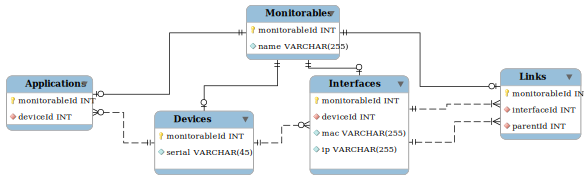
\includegraphics[width=0.9\textwidth]{contrib-asteroid-model}
		\caption{Exemple de schéma descriptif du réseau local domestique}\label{fig:contrib:asteroid:theorie:model}
	\end{figure}
\end{example}

La différence entre une donnée stable et une donnée statique est qu'il est intéressant de surveiller la modification d'une donnée (par des mécanismes tels que les \textit{triggers}) et en former un flux, qui peut être potentiellement archivé.

\textbf{Remarque} : Les clés artificielles ont une grande importance dans le cadre des applications d'observation. En effet, du fait du caractère incomplet de l'observation\footnote{soit parce que la donnée n'est pas parvenue au système, soit il n'existe pas de moyen technique pour y accéder}, il est possible d'obtenir des informations sur un équipement sans avoir pu obtenir son numéro de série. Des moyens alternatifs d'identification doivent être mis en place. Les clés artificielles permettent de tisser les relations entre les instances en ayant des données partielles. Toutefois, des vérifications d'intégrités sont nécessaires pour garder un modèle cohérent. Nous détaillons des cas applicatifs de ce problème dans nos expérimentations au chapitre~\ref{chap:valid:domvision}.

\subsubsection{Les historiques}
Supposons qu'une donnée \textit{volatile} est produite dans le flux $S$. Son historique est matérialisé par la relation temporelle $S[\infty]$. Il est nécessaire de faire persister la liste des historiques archivés. Nous modélisons cela par la création de l'association \textit{HasVolatile} donnant à partir d'un objet \textit{monitorable} et d'un \textit{volatile}, la relation contenant son historique.

D'un point de vue du schéma physique, les SGBD supportent rarement l'implémentation d'une relation dans un attribut. Pour contourner ce problème, nous créons une relation \textit{Pointers} indiquant un nom de relation historique et un attribut contenant la donnée \textit{volatile}. Ainsi, l'association \textit{HasVolatile} fournit un identifiant de pointeur au couple (\textit{monitorable, volatile}) comme montré dans la figure~\ref{fig:contrib:asteroid:theorie:volatile}.

\begin{figure}[ht]
    \centering
    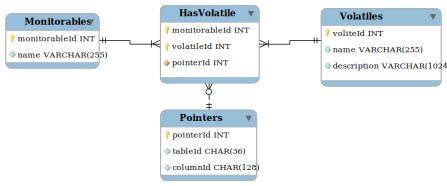
\includegraphics[width=0.8\textwidth]{contrib-asteroid-historians}
    \caption{Représentation physique de l'enregistrement des historiques}\label{fig:contrib:asteroid:theorie:volatile}
\end{figure}

\begin{example}
	Lors de l'enregistrement d'un historique de \textit{status} concernant un équipement par exemple, il est nécessaire d'insérer un n-uplet dans la relation \textit{Pointers}, qui permet de déclarer l'historique. Un autre est inséré dans \textit{HasVolatile} pour chaque \textit{monitorable} rencontré dans l'historique. Si la donnée \textit{status} n'avait pas été déclarée, il est nécessaire de le faire en insérant un n-uplet dans la relation \textit{Volatiles}.
	
	De façon similaire, les relevés de charges processeurs \textit{cpu} peuvent être attachés à un équipement ou à une application. Alors que les relevés de débits n'ont de sens que sur les interfaces (ou les liens suivant la modélisation voulue par l'utilisateur).
\end{example}

Il est intéressant de voir que puisque les données temps-réelles ont tendances à être de forte densité, il n'est peut-être pas possible de garantir une fraicheur des données au niveau du support de persistance pour les historiques.

\subsection{Représentation d'une relation persistante dans Astral}\label{sec:contrib:asteroid:theorie:astral}
Les relations issues d'un SGBD relationnel sont manipulables dans Astral du fait de leurs fondations théoriques similaires. Ainsi, une relation d'un système relationnel change au cours du temps, elle devient assimilable à une relation temporelle. Deux différences majeures subsistent : l'ordre des données et le mode d'interrogation.
\subsubsection{L'ordre d'une relation}
En SGBD, l'ordre n'importe pas jusqu'au moment de l'envoi des données à un utilisateur qui utilise le mot clé \textit{ORDER BY}. Le système peut en profiter pour modifier l'ordre lors d'opérations de jointures par exemple. Il est important de garder la même notion d'ordre au long de la requête continue. L'identifiant physique de la relation temporelle induite est par défaut la clé primaire de la relation persistante. Ainsi, nous gardons le même identifiant, et l'ordre est conservé lors des opérations.

\subsubsection{Le mode d'interrogation}
Afin d'être capable de représenter une relation temporelle dans \textit{Astronef}, il est nécessaire de pouvoir surveiller les changements effectués dans la relation persistante. Ceci peut toutefois être coûteux ou impossible suivant les moyens techniques disponibles dans le SGBD manipulé. Ainsi, pour être capable de représenter la relation telle que nous l'obtenons dans Astronef par la suite, nous utilisons un opérateur de manipulation du temps. Ce qui nous permet d'obtenir, comme indiqué dans la section~\ref{sec:contrib:astral:manipulation}, une mise à jour effective, périodique, à la demande ou inexistante.

Nous avons vu comment le SGBD peut être utilisé pour aider à la gestion de données d'observation. Nous avons aussi présenté comment représenter les relations persistantes dans Astral. Nous détaillons maintenant l'extension d'Astronef pour pouvoir manipuler le SGBD grâce à Astral.

\section{Composants Astronef}\label{sec:contrib:asteroid:composants}
\subsection{Source d'interrogation}
Comme présenté dans la section~\ref{sec:contrib:asteroid:theorie:astral}, une relation de base de donnée peut être présentée comme une relation temporelle Astral. Il est ainsi possible d'imaginer un composant source de donnée \textit{dbsource} capable de représenter une telle relation temporelle. Cette source devra suivre l'évolution de la relation suivant différents modes. Son implémentation est une application directe des principes exposés jusqu'ici : lorsque la relation temporelle doit être mise à jour, le composant interroge le SGBD avec une requête \textit{SQL} telle que \sql{SELECT * FROM Relation}.

Afin de pouvoir réutiliser \textit{dbsource}, nous pouvons le rendre plus générique en permettant la spécifications de paramètres de configuration. Ainsi, la source est capable de supporter la représentation de toutes requêtes du type $\D^f Q$ où $Q$ désigne une relation temporelle exprimable en algèbre relationnelle sur les relations de la base de donnée. La liste des paramètres de ce composants est disponible dans la table~\ref{tab:contrib:asteroid:dbsource} et la sémantique des modes de mise à jour est disponible dans la table~\ref{tab:contrib:asteroid:dbsource:modes}.
\begin{table}[ht]
    \centering
    \begin{tabular}{cl}
        paramètre & description \\ \midrule
        query & Requête \textit{SQL} à exécuter sur le SGBD \\
        mode & Sémantique de mise à jour
    \end{tabular}
    \caption{Paramètres obligatoires du composant \textit{dbsource}}\label{tab:contrib:asteroid:dbsource}
\end{table}
\begin{table}[ht]
    \centering
    \begin{tabular}{ccl}
        mode & sémantique & paramètre supplémentaire \\ \midrule
        hold & $\D^{\mathrm{id}}_{t\geq t_s}$ & \textit{at} : \textit{timestamp} correspondant à $t_s$ \\
        freeze & $\D^{\mathrm{freeze}^{t_s}}_{t\geq t_s}$ & \textit{at} : \textit{timestamp} correspondant à $t_s$\\
        trigger & $\D^{\mathrm{change}_{R_1,...,R_n}}$ & \textit{tables} : liste des relations $(R_i)$ à surveiller \\
        periodic & $\D^{\mathrm{period}^{r}}$ & \textit{rate} : période en seconde correspondant à $r$\\
        notify & $\D^{\mathrm{change}_{E}}$ & \textit{dependentRId} : identifiant du service de l'entité $E$
    \end{tabular}
    \caption{Modes supportés par le composants \textit{dbsource}}\label{tab:contrib:asteroid:dbsource:modes}
\end{table}

Il est important de voir que l'ensemble de la relation sera représenté dans la relation temporelle fournie. Or les relations temporelles sont placés en mémoires. Ainsi, si la séquence produite par l'interrogation du SGBD est de plusieurs millions d'n-uplets, le coût mémoire sera à prendre en compte. Comme cette source est capable de représenter toute requête \textit{SQL}, il est possible de déporter des opérations dans cette requête pour obtenir des résultats moins volumineux. Nous verrons dans la section~\ref{sec:contrib:asteroid:reecriture} comment effectuer cette opération automatiquement grâce à l'optimisation par règle d'Astronef.

\subsection{Macro-opération de jointure}
Le second composant d'Asteroid est un opérateur de jointure : \textit{dbjoin}. Son rôle est le suivant : lors de la réception d'un nouvel état d'une relation temporelle, requêter le SGBD et effectuer une jointure entre cet état et une requête \textit{SQL}. L'idée principale de cet opérateur est d'exploiter au maximum le SGBD. L'utilisation d'index pré-calculés sur le disque permet d'effectuer la jointure de façon efficace car l'optimiseur sélectionnera un plan performant grâce à ceux-ci.

D'un point de vue Astral, cet opérateur permet d'effectuer l'opération suivante $R \ssjoin_c Q$, où $Q$ est une relation temporelle exprimable en algèbre relationnelle sur les relations de la base de donnée, et $c$ une condition de jointure. Comme le composant \textit{dbsource}, il est configurables via les paramètres présentés dans la table~\ref{tab:contrib:asteroid:dbjoin}.
\begin{table}[ht]
    \centering
    \begin{tabular}{cl}
        paramètre & description \\ \midrule
        query & Requête \textit{SQL} à joindre sur le SGBD \\
        on & Expression de la condition de jointure (optionel)
    \end{tabular}
    \caption{Paramètres du composant \textit{dbjoin}}\label{tab:contrib:asteroid:dbsource}
\end{table}

Son implémentation peut différer selon les capacités fonctionnelles du SGBD. De façon générale, il est nécessaire d'utiliser une table temporaire \sql{Tmp} (en mémoire). Au moment de l'exécution de \textit{dbjoin}, l'opérateur insère les données de la séquence fournie dans \sql{Tmp}. Ensuite, il applique la requête \textit{SQL} suivante : \begin{center} \sql{SELECT * FROM Tmp AS l NATURAL JOIN (*query*) AS r ON (*on*)} \end{center}
Le résultat est transformé en séquence d'n-uplet qui sera envoyée à la relation temporelle de sortie. La requête \sql{DELETE FROM Tmp} est ensuite appliqué pour supprimer les données temporaires. Par mesures de performances évidentes, les requêtes sont préparés à l'avance pour ne plus avoir le coût de préparation du plan.

Sur certains SGBD, il est possible d'optimiser cette implémentation. Sur \textit{H2} par exemple, il est possible d'utiliser la syntaxe \sql{TABLE(A1 T1=?,...,An Tn=?)} pour représenter une table temporaire d'attributs $A_i$ et de types $T_i$ dont les données seront passés comme paramètres lors de l'exécution de la requête. Il est aussi possible d'accélerer l'opération de suppression via l'opération \sql{TRUNCATE} maintenant répendue parmis les SGBD populaires.

\subsection{Composants puits de persistance}

\section{Plan d'exécution}\label{sec:contrib:asteroid:reecriture}

\section{Conclusion}
Ce chapitre a dressé un état de l'art des différents systèmes capables d'offrir une solution générique de supervision. Il en ressort qu'aucun système ne supporte entièrement les critères de qualité que nous nous sommes fixés. Le tableau~\ref{tab:rw:supervision:bilan} résume les 11 points d'analyse en colorant les différentes points suivant leurs conformités. 

\begin{sidewaystable}[ht]
\centering
\begin{tabular}{@{{\vrule width 1pt}\ \ }>{\raggedleft}m{3cm}@{\ \ {\vrule width 1pt}\ \ }M{4.2cm}|M{4.2cm}|M{4.2cm}|M{4.2cm}@{\ \ {\vrule width 1pt}}} \bottomrule
\head Critère & \head Système d'administration & \head Gestion de contexte & \head Entrepôts de données & \head Gestion de flux de données \\  \toprule \bottomrule
\critereAA & Hiérarchique & Triplets & Relationnel & Relationnel dérivé \\ \hline
\critereAB & \meh Structure hiérarchique sans contraintes & \good Ontologies & \good Modèle relationnel normalisé & \bad Pas de structure \\ \hline
\critereAC & \meh Notifications & \bad Ajout du temps en propriété & \meh CDC & \good Flux natif \\ \toprule \bottomrule
\critereBA & \meh Instantanée, continu en ad-hoc & \bad Instantané principalement & \meh Instantané. ETL en pseudo-continu & \bad Continu uniquement \\ \hline
\critereBB & \good Standardisation, union de modèles & \meh Fusion d'ontologies non standardes & \good Processus ETL (complexe) & \good Union et jointures de flux \\ \hline
\critereBC & \bad Impératif principalement & \good Logique & \meh Déclaratif (SQL) et Procédural (ETL) & \good Déclaratif principalement\\ \hline
\critereBD & \meh Procédures à écrire soi-même & \good Logique du premier ordre & \good Relationnel multidimensionnel et Algorithmie dédiée & \meh Relationnel avec support du dynamisme\\ \toprule \bottomrule
\critereCA & \good Support des standards & \meh Spécification longue des domaines & \bad Spécification du schéma, des ETL, autre (complexe) & \good Écriture de requêtes \\ \hline
\critereCB & \bad Aucune & \good Séparation par les domaines & \good Données multidimensionnelles & \bad Aucune \\ \hline
\critereCC & \good Modèle extensible, fonctions métiers dans le gestionnaire & \meh Capteurs virtuels & \good Opérateurs ETL, procédures SQL, algorithmes & \meh Sources et puits mais pas les opérateurs  \\ \hline
\critereCD & \good Large échelle & \bad Complexité très haute & \meh Réactivité lente, Support de grande quantité & \good Support de haut débits\\ \toprule 
\end{tabular}
\caption{Récapitulatif de l'état de l'art des systèmes génériques de supervision}\label{tab:rw:supervision:bilan}
\end{sidewaystable}
Il en ressort que les systèmes d'administrations sont avant tout des systèmes qui fonctionnent grâce au support des standards et à leur simplicité d'implémentation. L'architecture avec gestionnaire adaptable grâce à des langages impératifs permets une grande flexibilité pour s'adapter aux cas d'usages. De son côté, l'informatique contextuelle fournit des outils permettant de modéliser et manipuler proprement les concepts du système grâce aux ontologies et aux raisonnements logiques. Il en sort une claire séparation des domaines de compétences. Les entrepôts de données quant à eux se distinguent par des capacités d'analyses très poussées, ainsi qu'un procédé d'intégration, très complexe et lourd malheureusement, mais très complet. Enfin, la gestion de flux de données est une base solide pour gérer les données dynamiques. L'intégration et l'adaptation au système étant fait entièrement de manière déclarative en fait une solution performante et viable.

À la vue de l'état de l'art, voici les points qui vont être critique sur notre établissement de notre contribution :
\begin{itemize}
    \item La gestion de flux est un bon socle pour gérer les données dynamique grâce aux requêtes continues.
    \item Elle ne suffit pas pour constituer un système d'observation complet, notamment à l'absence de modèle de description et de requêtes instantanées.
    \item Les entrepôts et bases de données sont capables de répondre aux requêtes instantanées.
    \item Les ETL sont trop complexes à manipuler pour intégrer les données, alors que les SGFD sont plus déclaratifs.
\end{itemize}
Il devient clair que les systèmes de gestions de flux de données forment un bon candidat comme fondation pour un architecture d'observation de système. Il nous faut donc approfondir l'état de l'art technique sur ce domaine pour modeler notre contribution. Le point majeur sera d'apporter les capacités des systèmes de gestions de données relationnels. En effet, en apportant le support persistant à la gestion de flux de données, en clarifiant et augmentant son langage, nous aurons un outil qui sera plus apte à répondre à notre problématique. Ainsi, l'héritage du relationnel permettra une structure sémantique correcte, ainsi que des capacités d'analyses plus évoluées. Enfin et surtout, les données serait intégrés malgré leur hétérogénéité profonde. Le chapitre suivant détaille l'état de l'art technique de la gestion de flux de données afin de pouvoir effectuer ces améliorations.

\chapterhead{Table des règles Astronef}
\listofreglefloat

